% !TEX root = BIGALL-Master.tex
\section{Theoretische Grundlagen}
\subsection{Synthese von Nanopartikeln}
	Bei der Herstellung von Nanopartikeln wird zwischen der \glqq bottom-up\grqq - und der \glqq top-down\grqq - Methode unterschieden.
	Bei der \glqq top-down\grqq - Methode wird mit einem Festkörper angefangen, der dann durch verschiedene physikalische Zerkleinerungsmethoden (wie z.B. Kugelmühlen oder Laser) auf eine gewünschte Partikelgröße gebrochen wird.
	Da diese Brüche nicht gleichmäßig stattfinden, eignen sich diese Methoden weniger um monodisperse Nanokristalle herzustellen, wenn eine sehr schmale Größenverteilung gebraucht wird.
	Bei der \glqq bottom-up\grqq - Methode wird ein Nanopartikel aus vielen Monomeren zusammengesetzt, bis zur gewünschten Größe.
	Diese Methode kann mit einzelnen Klemmbausteinen verglichen werden, die zu größeren Gebilden zusammengesetzt werden können.
	Da man bei diesem Verfahren viele Parameter hat, die verändert werden können, durch die die Partikeleigenschaften beeinflusst werden, bietet sich das \glqq bottom-up\grqq - Verfahren zur Synthese monodisperser Partikel besser an, da durch die richtige Abstimmung der Parameter ein kontrolliertes Nukleationsverhalten und späteres Wachstum erreicht werden können.
	Parameter, die eingestellt werden können sind u.a. Reaktionstemperatur und Dauer, Konzentration der Edukte, Druck oder Lösungsmittel.
	
	Die theoretische Beschreibung der Bildung monodisperser Nanopartikel geht auf Untersuchungen von LaMer und Dinegar zurück.\autocite{Lamer1950}
	Sie zeigten, dass die Bildung
	monodisperser Kristalle eine zeitlich diskrete (nicht kontinuierliche) Keimbildung
	erfordert, gefolgt von einem langsameren kontrollierten Wachstum der existierenden
	Kerne.
	Bei dem Konzept der sog. „schlagartigen Keimbildung“ muss demnach die
	Keimbildung zu einem einzigen Zeitpunkt ausgelöst werden. Weitere
	Keimbildungsereignisse sind auszuschließen. Startend in einer homogenen Phase setzt
	bei Überwindung der Energiebarriere die Keimbildung ein und es resultiert eine
	heterogene Phase unter homogener Nukleation. \autocite{Park2007}
	
	\begin{figure}[H]
		\centering
		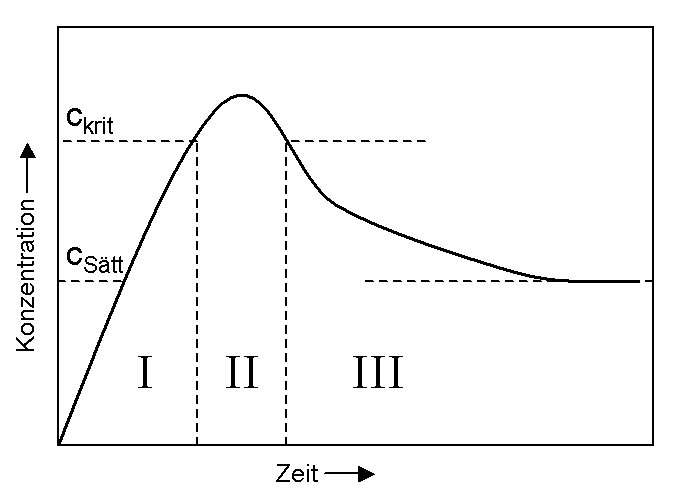
\includegraphics[width=0.6\textwidth]{Bilder/LaMer} 	
		\caption{LaMer-Diagramm: Monomerkonzentration als Funktion der Zeit.\autocite{Lamer1950}}
		\label{fig:LaMer}
	\end{figure}

	Im LaMer-Modell existieren ,wie in \cref{fig:LaMer} gezeigt, 3 Stufen. 
	In Stufe I ist eine kontinuierliche Zunahme der Monomerkonzentration dargestellt.
	Durch die Energiebarriere kommt es auch nach Überschreiten der Sättigungs-Konzentration $C_{Sätt}$ zu keiner Keimbildung.
	Zum Erreichen der Keimbildung in Stufe II muss eine kritische Konzentration $c_{krit}$ überschritten werden.
	Hier werden schlagartig Keime gebildet mit einem kritischen Radius $r_{krit}$, wodurch die Monomerkonzentration wieder unter $c_{krit}$ sinkt, wo dann keine weiteren Keime mehr gebildet werden können.
	
	$r_{krit}$ muss erreicht werden, da aufgrund der energetisch ungünstigen Lage von Atomen auf der Oberfläche von Nanopartikeln Kristallkeime unterhalb von $r_{krit}$ nicht stabil sind und dissoziieren.
	Die Änderung der freien Enthalpie $\Delta G$ bei der homogenen Nukleation setzt sich dabei additiv aus einem Volumenanteil und einem Oberflächenanteil zusammen, der unter Annahme einer kugelförmigen Nukleation in \cref{eq:1} gezeigt ist.\autocite{Thanh2014}
	\begin{equation}
	\label{eq:1}
	\Delta G = 4 \pi r^2 \gamma + \dfrac{4}{3} \pi r^3 \Delta G_V
	\end{equation}
	Dabei ist $\gamma$ die Oberflächenergie, $r$ der Radius des Partikels und $\Delta G_V$ die freie Enthalpie des Kristalls, die in \cref{eq:2} gegeben ist und wiederum von der Übersättigung der Lösung $S$, dem molaren Volumen $v$, der Temperatur $T$ und der \textsc{Boltzmann}-Konstante $k_B$ abhängt.
	\begin{equation}
	\label{eq:2}
	\Delta G_V = \dfrac{-k_B T ln(S)}{v}
	\end{equation}
	Dadurch ergibt sich insgesamt für die freie Enthalpie $\Delta G$:
	\begin{equation}
	\Delta G = \dfrac{4}{3} \pi r^3 \dfrac{-k_B T ln(S)}{v}+4 \pi r^2 \gamma
	\end{equation}
	 
	Durch die entgegengesetzten Vorzeichen vom Flächen- und Volumenanteil ergibt sich ein energetisches Maximum, das überwunden werden muss, damit die Keime nicht wieder dissoziieren.
	Dies ist grafisch in \cref{fig:Keimbildung} gezeigt 
	
	\begin{figure}[H]
		\centering
		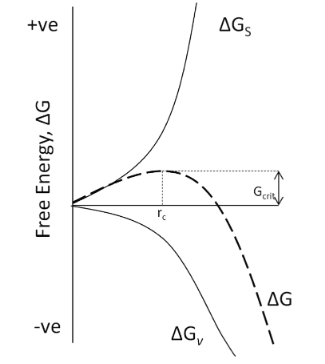
\includegraphics[width=0.6\textwidth]{Bilder/Keimbildung} 	
		\caption{Diagramm der freien Enthalpie  $\Delta G$ resultierend aus Oberflächenanteil  $\Delta G_S$ und Volumenanteil  $\Delta G_V$.\autocite{Thanh2014}}
		\label{fig:Keimbildung}
	\end{figure}
	Daraus folgt für den kritischen Radius $r_{krit}$:
	\begin{equation}
	r_{krit}=\dfrac{2 \gamma v}{k_B T ln(S)}
	\end{equation}
	
	Nach der Keimbildung wird dann Stufe III erreicht, bei der die Monomere nicht mehr zur Keimbildung, sondern zum Wachstum der Keime genutzt werden, bis ein Gleichgewichtszustand bei der Sättigungskonzentration erreicht wird.
	
%----------------------------------------------
	
	\subsection{Halbleiternanopartikel \& Größenquantisierungseffekt}
	Während Halbleiter als Festkörper eine feste Bandlücke zwischen Valenz- und Leitungsband aufweisen, ist sie bei Nanopartikeln eine von der Partikelgröße abhängige Eigenschaft.
	Allgemein gilt, dass bei kleineren Partikeln die Bandlücke zunimmt.
	\begin{figure}[h]
		\centering
		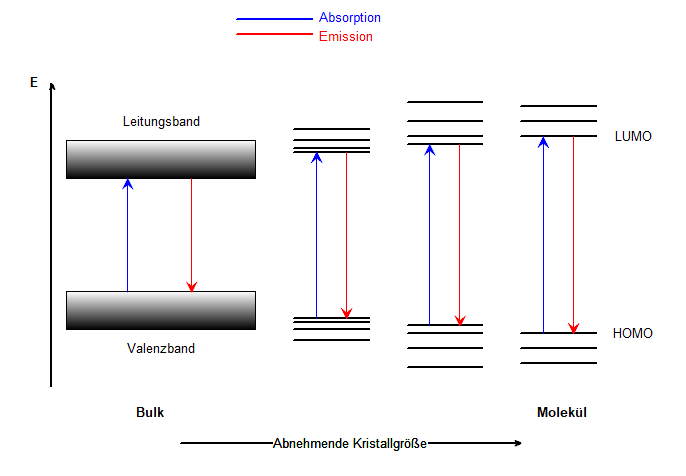
\includegraphics[width=0.6\linewidth]{Bilder/Quantumsizeeffect}
		\caption{Schematische Darstellung der Veränderung der Bandlücke bei abnehmender Kristallgröße.}
		\label{fig:LCAO}
	\end{figure}
	
    Dies lässt sich über 2 Theorien beschreiben. Zum einen auf der Basis des LCAO-Modells (Linear Combination of Atomic Orbitals) bei dem Nanopartikel als große Moleküle gesehen werden, zum anderen auf Basis der Festkörpertheorie, die Nanopartikel als kleine Festkörper beschreibt.
	
	Bei der LCAO-Methode bilden $n$ Atomorbitale, die gleiche Symmetrie und ähnliche Energie besitzen, durch lineare Kombination, $n$ Molekülorbitale. Wird $n$ sehr groß, kommt es zu einer großen Anzahl Energieniveaus, die sehr nahe beieinander liegen, wodurch kontinuierliche Energiebänder entstehen.
	Bei Isolatoren und Halbleitern gibt es eine Bandlücke zwischen den Bändern, die bei großen Festkörpern, bei denen die Annahme $n \rightarrow \infty$  gilt, zu einer festen Materialeigenschaft führt.
	Der Unterschied zwischen Isolator und Halbleiter ist dabei die Größe der Bandlücke, so werden Materialien mit einer Bandlücke von bis zu 4~eV meist den Halbleitern zugeordnet und Materialien mit einer größeren Bandlücke zu den Isolatoren.
	Bei Nanopartikeln gilt die Näherung $n \rightarrow \infty$ allerdings nicht mehr, wodurch sich die kontinuierlichen Bänder mit sinkender Anzahl Atomen wieder in diskrete Energieniveaus aufteilen. Dabei vergrößert sich auch die Bandlücke wieder, wie in \cref{fig:LCAO} dargestellt.
	
	Bei der Festkörpertheorie kommt es zur Absorption eines Photons, wodurch ein Elektron $e^{-}$ vom Valenzband ins Leitungsband angeregt wird.
	Daraus resultiert ein Loch $h^{+}$  im Valenzband. 
	Aufgrund der unterschiedlichen Polarität von Loch und Elektron ziehen sich diese gegenseitig an. 
	Dies bewirkt, dass sich Elektron und Loch nicht frei im Partikel bewegen können, sondern ein Elektron-Loch-Paar bilden, das Exziton genannt wird. 
	Der durchschnittliche Abstand von $e^{-}$ und $h^{+}$ wird Exziton-Bohr-Radius genannt.
	In einem Nanopartikel ist die Bewegung durch die Partikelgrenzen beschränkt, die als Potentialgrenzen wirken, ähnlich des „Teilchen im Kasten“-Modells, bei dem das Potential außerhalb unendlich ist.
	Ist die Partikelgröße kleiner als der Exziton-Bohr-Radius, muss somit die Bandlücke steigen.
	Die Änderung der Bandlücke mit dem Partikelradius unter Berücksichtigung der  Coulombwechselwirkung zwischen Elektron und Loch wird durch die \textsc{Brus}-Formel beschrieben:\autocite{Brus1984}
	
	\begin{equation}
	\label{eq:BRUS}
	E_{NC}=E_{g}+\frac{h^{2}}{8R^{2}}\left( \frac{1}{m^{*}_{e}}+\frac{1}{m^{*}_{h}}\right)-\frac{1,8e^{2}}{4\pi\epsilon_{0}\epsilon_{r}R} 
	\end{equation}
	\begin{multicols}{2}
		\begin{flushleft}
			$E_{NC}$:	Bandlücke des Nanokristalls\\
			$E_{g}$:	Bandlücke des Festkörpers\\
			$h$:		Plank´sches Wirkungsquantum\\
			$R$:		Partikelgröße\\
			$m^{*}_{e}$: Effektive Masse des $e^{-}$\\
			$m^{*}_{h}$: Effektive Masse des $h^{+}$\\
			$\epsilon_{0}$: Permittivität des Vakuums\\
			$\epsilon_{r}$: relative Permittivität\\
			$e$: Elementarladung\\
		\end{flushleft}
	\end{multicols}
	
%-----------------------------------------------------

    \subsection{Metallnanopartikel \& Oberflächenplasmonen}
    
    Metallische Nanopartikel, die kolloidal in Lösung vorliegen, zeigen meist ein charakteristisches Absorptionsspektrum.
    Dieses ist aber anders als bei Halbleitern nicht auf Elektronenübergänge zwischen quantisierten Energiezuständen einzelner Elektronen zurückzuführen, sondern es kommt zu einer kollektiven Anregung eines Elektronenensembles.
    Diese Anregung wird als Oberflächenplasmonenresonanz bezeichnet. \autocite{Mulvaney1996}
    Durch die Absorption durch ganze Elektronenensembles und nicht durch einzelne Elektronen ist der Absorptionskoeffizient dieser Partikel sehr stark, wodurch auch stark verdünnte Lösungen immer noch eine intensive Färbung aufweisen können. 
    
    Das Phänomen der lokalisierten Oberflächenplasmonenresonanz (LOPR) entsteht bei der Wechselwirkung von einer elektromagnetischen Welle und frei beweglichen Elektronen eines Metallnanopartikels.\autocite{Hu2006}
    Das periodische elektromagnetische Feld verursacht dabei eine kollektive Oszillation der leitenden Elektronen, wenn die passende Resonanzfrequenz getroffen wird.
    Da die absorbierten Photonen in Phonen des Metallgitters umgewandelt werden, kann kein Emissionsspektrum gemessen werden.
    Für Nanopartikel mit einem Radius $r<<\lambda$, mit $\lambda$ als Wellenlänge, kann in guter Näherung ein, das Partikel durchdringende Feld, als homogen über das gesamte Partikel angenommen werden (\cref{fig:LOPR}). \autocite{Xu1999}
    Dadurch kann vereinfacht angenommen werden, dass bei $r<<\lambda$ nur die Dipolanregung zur Extinktion beiträgt und die Dipolaufspaltung als quasistatisch angenommen werden kann. 
    Bei Gold liegt dieser Bereich bei $\approx$2-30~nm.
    
    \begin{figure}[H]
        \centering
        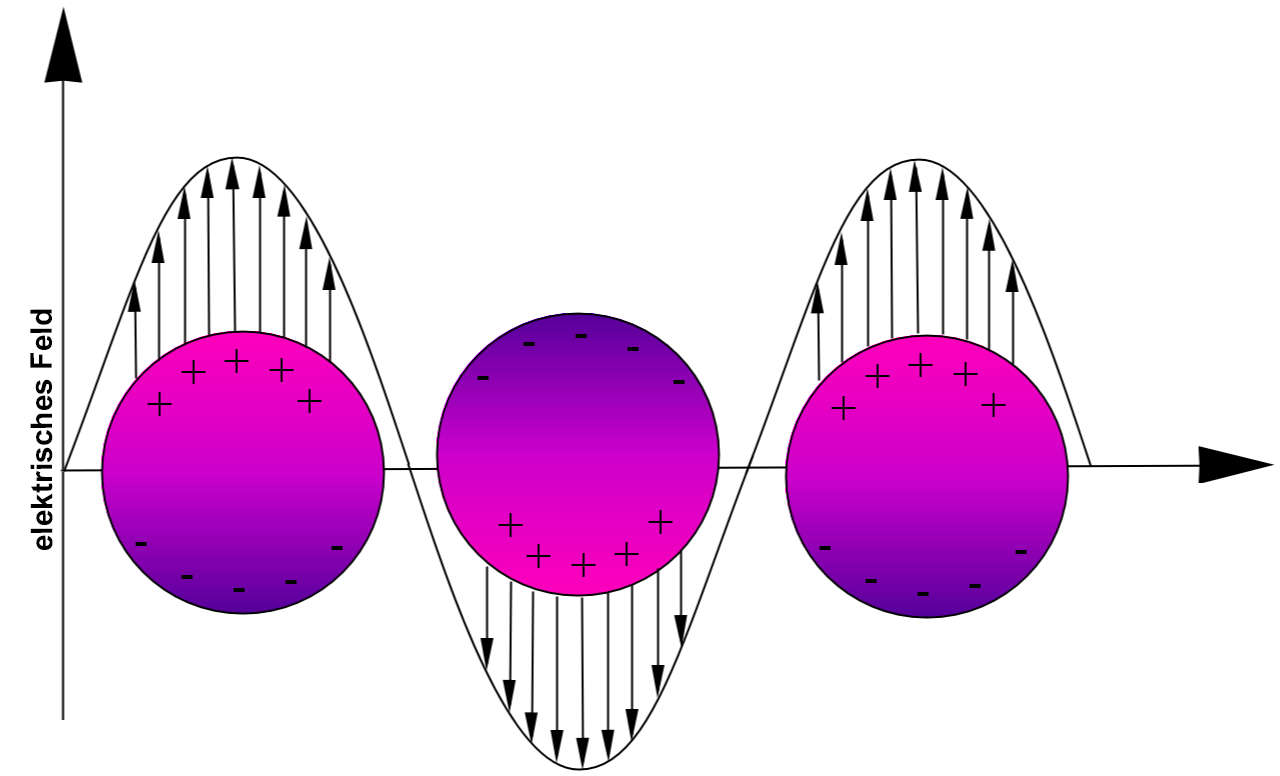
\includegraphics[width=0.6\linewidth]{Bilder/LSPR}
        \caption{Schematische Darstellung der lokalisierten Oberflächenresonanz (LOPR).}
        \label{fig:LOPR}
    \end{figure}
    
    Die plasmonische Resonanzfrequenz ist dabei durch die Permittivität des Metalls, die Größe und Form des Partikels und die Permittivität des umgebenden Mediums beeinflussbar. \autocite{Kelly2003,Mock2003}
    Die LOPR-Bande dieser Partikel können sich vom ultravioletten bis in den infraroten Bereich erstrecken. \autocite{Haes2004}
    
    \subsection{Metall-Halbleiter-Nanopartikel}
    Wenn Metallpartikel in der Nähe von fluoreszierenden Halbleiter-Nanopartikeln liegen haben diese Einfluss auf die Fluoreszenz dieser.
    Die plasmonischen Metallnanopartikel können als optische Antennen aufgefasst werden, sie können also die zur Anregung der LOPR einfallenden Strahlung im Nahfeld lokalisieren. 
    Je nach Abstand zwischen beiden kann es sowohl zu Fluoriszenzverstärkung als auch zu Fluoriszenzauslöschung kommen. \autocite{Kulakovich2002,Viste2010}
    
    Die Verstärkung kann hauptsächlich auf den Anstieg der Anregungsrate im Fluorophor zurückgeführt werden.\autocite{Chen2008}
    Eine Verstärkung kann durch die chemische Kupplung mit definierten Abstand von plasmonischen Partikeln an die Oberfläche der Halbleiter-Nanopartikel erreicht werden.\autocite{Lee2004}
    
    Die Auslöschung wird durch sehr geringe Abstände oder eine direkte chemische Bindung verursacht.\autocite{Costi2010}
    Hier kommt es durch die direkte Verbindung der unterschiedlichen Domänen an der Metall-Halbleiter-Grenzfläche zu einem Ladungstransfer und somit zu einer Ladungstrennung.
    Hierbei wird ein angeregtes Elektron aus dem Leitungsband des Halbleiters in die Metalldomäne übertragen.
    Dies ist dann möglich, wenn sich das Fermi-Niveau des Metalls innerhalb der Bandlücke des Metalls befindet (\cref{fig:Ladungstrennung}).
    Durch die direkte Übertragung der angeregten Elektronen aus dem Leitungsband des Halbleiters auf das Fermi-Niveau des Metalls, erhöht sich zum einen die Menge an strahlungsfrei relaxierter Ladung, zum anderen wird dadurch die Verkürzung der Lebensdauer des angeregten Zustands bedingt.\autocite{Banin2014}
    \begin{figure}[H]
    	\centering
    	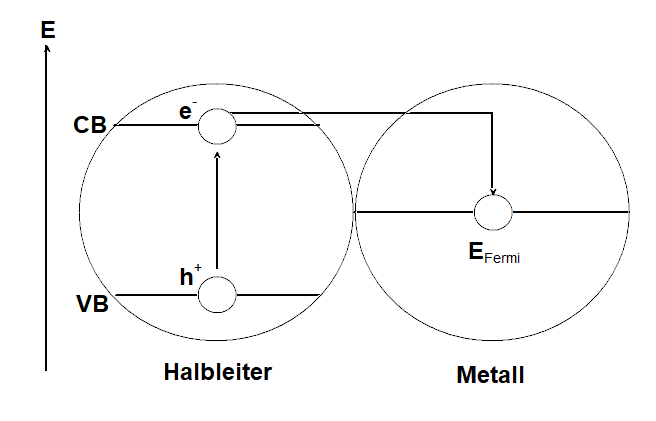
\includegraphics[width=0.6\textwidth]{Bilder/HL-M} 	
    	\caption{Ladungsträgertrennung an einer Metall-Halbleiter-Grenzfläche.}
    	\label{fig:Ladungstrennung}
    \end{figure}
    
    
    \subsection{Nanopartikelbasierte Gele}
    
    Allgemein sind Gele Systeme aus mindestens zwei Komponenten, wobei eines ein festes dreidimensionales Netzwerk bildet und von einer Flüssigkeit oder einem Gas ausgefüllt ist. \autocite{Aleman2007}
    
    Der klassische Bildungsmechanismus folgt meist dem Sol-Gel-Verfahren. \autocite{Ziegler2017}
    Dabei wird aus einem flüssigen System über stufenweise Umwandlungen von Vorstufen ein Sol gebildet woraus anschließend ein Gel entsteht. \autocite{Aleman2007}
    Diese Umwandlungen sind meist Polymerisationsreaktionen oder bei anorganischen, oxidschen Gelen Kondensationsreaktionen. 
    Da bei diesen Reaktionen das Material, das das Sol und später das Netzwerk bildet, das gleiche ist, wie das verknüpfende, können diese Prozesse nur für spezielle Materialien durchgeführt werden.
    
    Da viele Eigenschaften von Nanopartikeln form- und größenabhängig sind, diese aber bei diesem klassischen Ansatz nur schwer bis gar nicht einstellbar sind für Goldnanopartikel, eignet er sich für diese Gelierung nicht.
    
    Dieses Problem konnte erstmals in der Arbeit von Brock und Monahan 2004 umgangen werden, durch kontrollierte Destabilisierung und Trocknung der Nanopartikel. \autocite{Mohanan2004,Mohanan2005}
    Diese Destabilisierung erfolgt durch Zugabe eines Oxidationsmittels in eine Lösung von ligandenstabilisierten Nanopartikeln.
    Durch diese Zugabe reagieren Teile der Liganden miteinander, wodurch es  an der Oberfläche der Nanopartikel zu freiliegenden Bereichen kommt, an denen die Partikel dann aggregieren können.
    Neben diesem Ansatz sind auch andere Gelierungsstrategien bekannt, die in \cref{fig:Destabilisierung} gezeigt sind, wie z.B. die Änderung der Polarität vom Lösungsmittel, was zur Veränderung des Zeta-Potentials und so zur Destabilisierung der Kolloide führt, was so zur Gelbildung führen kann.
    
    \begin{figure}[H]
        \centering
        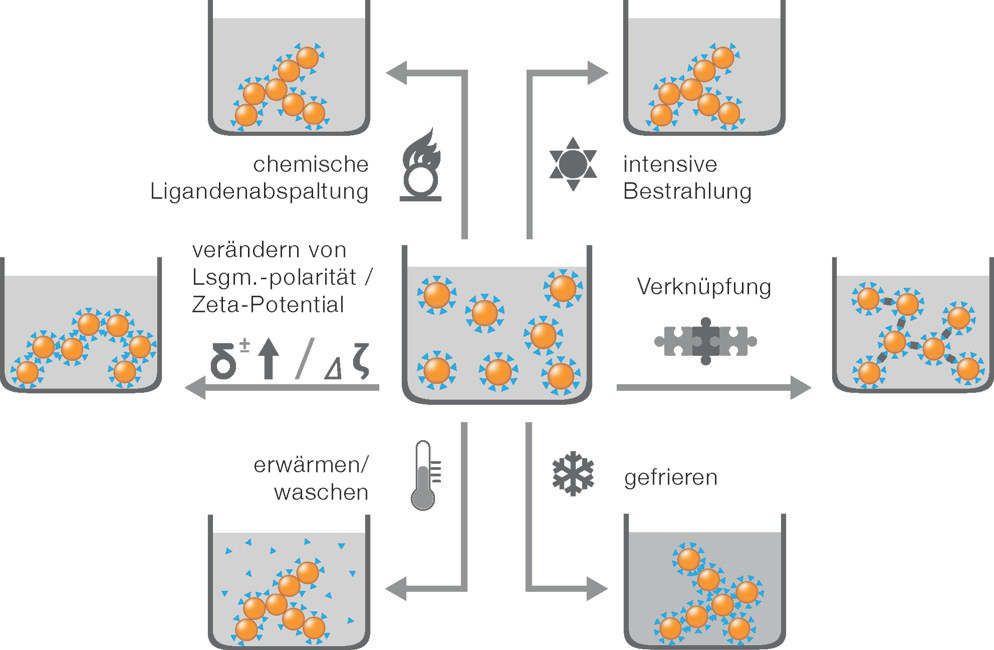
\includegraphics[width=0.6\linewidth]{Bilder/Gelierung.png}
        \caption{Strategien für die kontrollierte Destabilisierung von vorab gebildeten kolloidalen Lösungen.\autocite{Aleman2007}}
        \label{fig:Destabilisierung}
    \end{figure}
    
    Auf diese Weise können auch metallische Nanopartikel zu Gelen weiterverarbeitet werden. \autocite{Bigall2009}
    Diese zeigen vielversprechende Eigenschaften bei verschiedenen elektrokatalytischen Prozessen wie Alkoholoxidation, Sauerstoffreduktionsreaktion und Sauerstoffentwicklungsreaktion.  \autocite{Cai2018,Shi2018,Zhu2016,Shi2017,Wang2019}
    Die Gele sind dabei auch besonders interessant, da sie ein sehr großes Oberfläche-zu-Masse-Verhältnis besitzen, was eine hohe katalytische Wirkung bei wenig eingesetztem Material bewirkt. 
    Edelmetall-Nanostrukturen weisen einzigartige optische Eigenschaften auf, die eine Kopplung zwischen den kollektiven Oberflächenelektronenoszillationen und dem einfallenden elektromagnetischen Feld ermöglichen und so ein dramatisch verstärktes lokales elektrisches Feld für eine oberflächenverstärkte Raman-Streuung ergeben. \autocite{Linic2015,Gao2016}

    
    \subsection{Metall-Halbleiter-Gele}
    Im Gegensatz zu den in dieser Arbeit untersuchten Gelen, bei denen Metallnanopartikelgele mit Halbleitern modifiziert werden, sind die bisherigen Untersuchungen auf diesem Gebiet der Metall-Halbleiter-Gele von Halbleitergelen ausgegangen, die dann mit Metallnanopartikeln wie Gold oder Silber modifiziert wurden. \autocite{Nahar2015,Lesnyak2011} 
    Bei den bisherigen Untersuchungen konnten Emissionen beobachtet werden mit Zerfallsraten,  die beim reinen Halbleitergel nicht beobachtet werden können, was auf die Erzeugung alternativer Strahlungszerfälle hinweist. \autocite{Nahar2015}
    Gleichzeitig konnte bei höheren Raten an Metallpartikel eine Fluoreszenzauslöschung beobachtet werden. \autocite{Lesnyak2011}
    